\section{Our Approach}
Our motivation in this paper is to propose a method with minimal feature engineering effort to solve target type identification. For this task, we use the test collection introduce in \cite{Garigliotti:2017:TTI:3077136.3080659}. In this test collection, for a given query there is a pool of target entity types. for each target type in the pool, there is a label between zero (non-relevant) and seven (the most relevant) which indicate the relevance degree of the query and that target type. Similar to the propose LTR approach in \cite{Garigliotti:2017:TTI:3077136.3080659} we cast the type identification problem into regression problem i.e for a given pair of query and type the goal is to predict the relevancy score.

Following the idea of TC and EC method introduce in \label{key} we defined two matrices i.e $I_{TC}$ and $I_{EC}$ that models word level similarities via word embeddings. 

\boldsymbol{$I_{TC}:$} For a given query-type pair $(q,t)$, we first extract top-50 words representing type $t$. These words are selected according to the tf.idf score. We then build $I_{TC}$ matrix as follows. Each row of matrix indicates a query term (e.g $q_i$) of $q$ (in order of occurrence) and each column of the matrix indicates a representing word (e.g $w_j$) of that type (sorted by tf.idf score). The entry $I_{TC}[i,j] = cos(\vec{q_i}, \vec{w_j})$ where $\vec{q_i}$ and $\vec{w_j}$ indicates the pre-trained word embedding vectors of \cite{Mikolov:2013:DRW:2999792.2999959}.

\boldsymbol{$I_{EC}:$} For a given query-type pair $(q,t)$, we first used a language retrieval model to retrieve top-20 ranked entities (i.e $e_1,\cdots, e_{20}$) for query $q$. $I_{EC}$ is made by concatenation of twenty matrices as $I_{EC} = [I_{E_1C},\cdots, I_{E_{20}C}]$ where $I_{E_iC}$ is a matrix indicating the relevancy of query $q$ and entity $e_i$ considering the type $t$. Each entry of matrix $I_{E_iC}$ is computed as follows:
\begin{equation}
I_{E_iC}[m,n] = 
\begin{cases}
cos(q_m,w_{i,n}) \times W(e,t) &\quad\text{type(e)} \cap t \neq \phi \\
0 &\quad\text{otherwise} \\
\end{cases}
\end{equation}
Where $q_m$ is the $m^{\text{\tiny th}}$ query term and $w_{i,n}$ ($1\leq n \leq20$) indicates the $n^{\text{\tiny th}}$ word (sorted on tf.idf score) representing the entity $e_i$. $W(e,t)$ is the function  described in section \ref{EC} and $type(e)$ is the set of types associate with entity $e$.


In our first attempt to solve the problem we use two feedforward neural networks. the input of these networks are $I_{TC}$ and $I_{EC}$, respectively.


Similar to the translation, rotation and scale invariance of images in CNN, CNN is able to learn the local features from words or phrases in different places of text \cite{wang2016combination}. As a result, in our second attempt, we present a jointed convolutional neural network and feedforward (FF) architecture that takes the local features extracted by CNN as input to FF for target type identification problem. We try this architecture twice with $I_{EC}$ and $I_{TC}$ as the inputs of the CNN models, respectively.

Finally, following the idea of combining entity centric and type centric models\cite{Balog:2011:QME:2037661.2037667,Garigliotti:2017:TTI:3077136.3080659}, we propose the architecture represented in fig.\ref{proposeModel}. This architecture is the combination of the above mentioned CNN+FF networks.
\begin{figure*}
	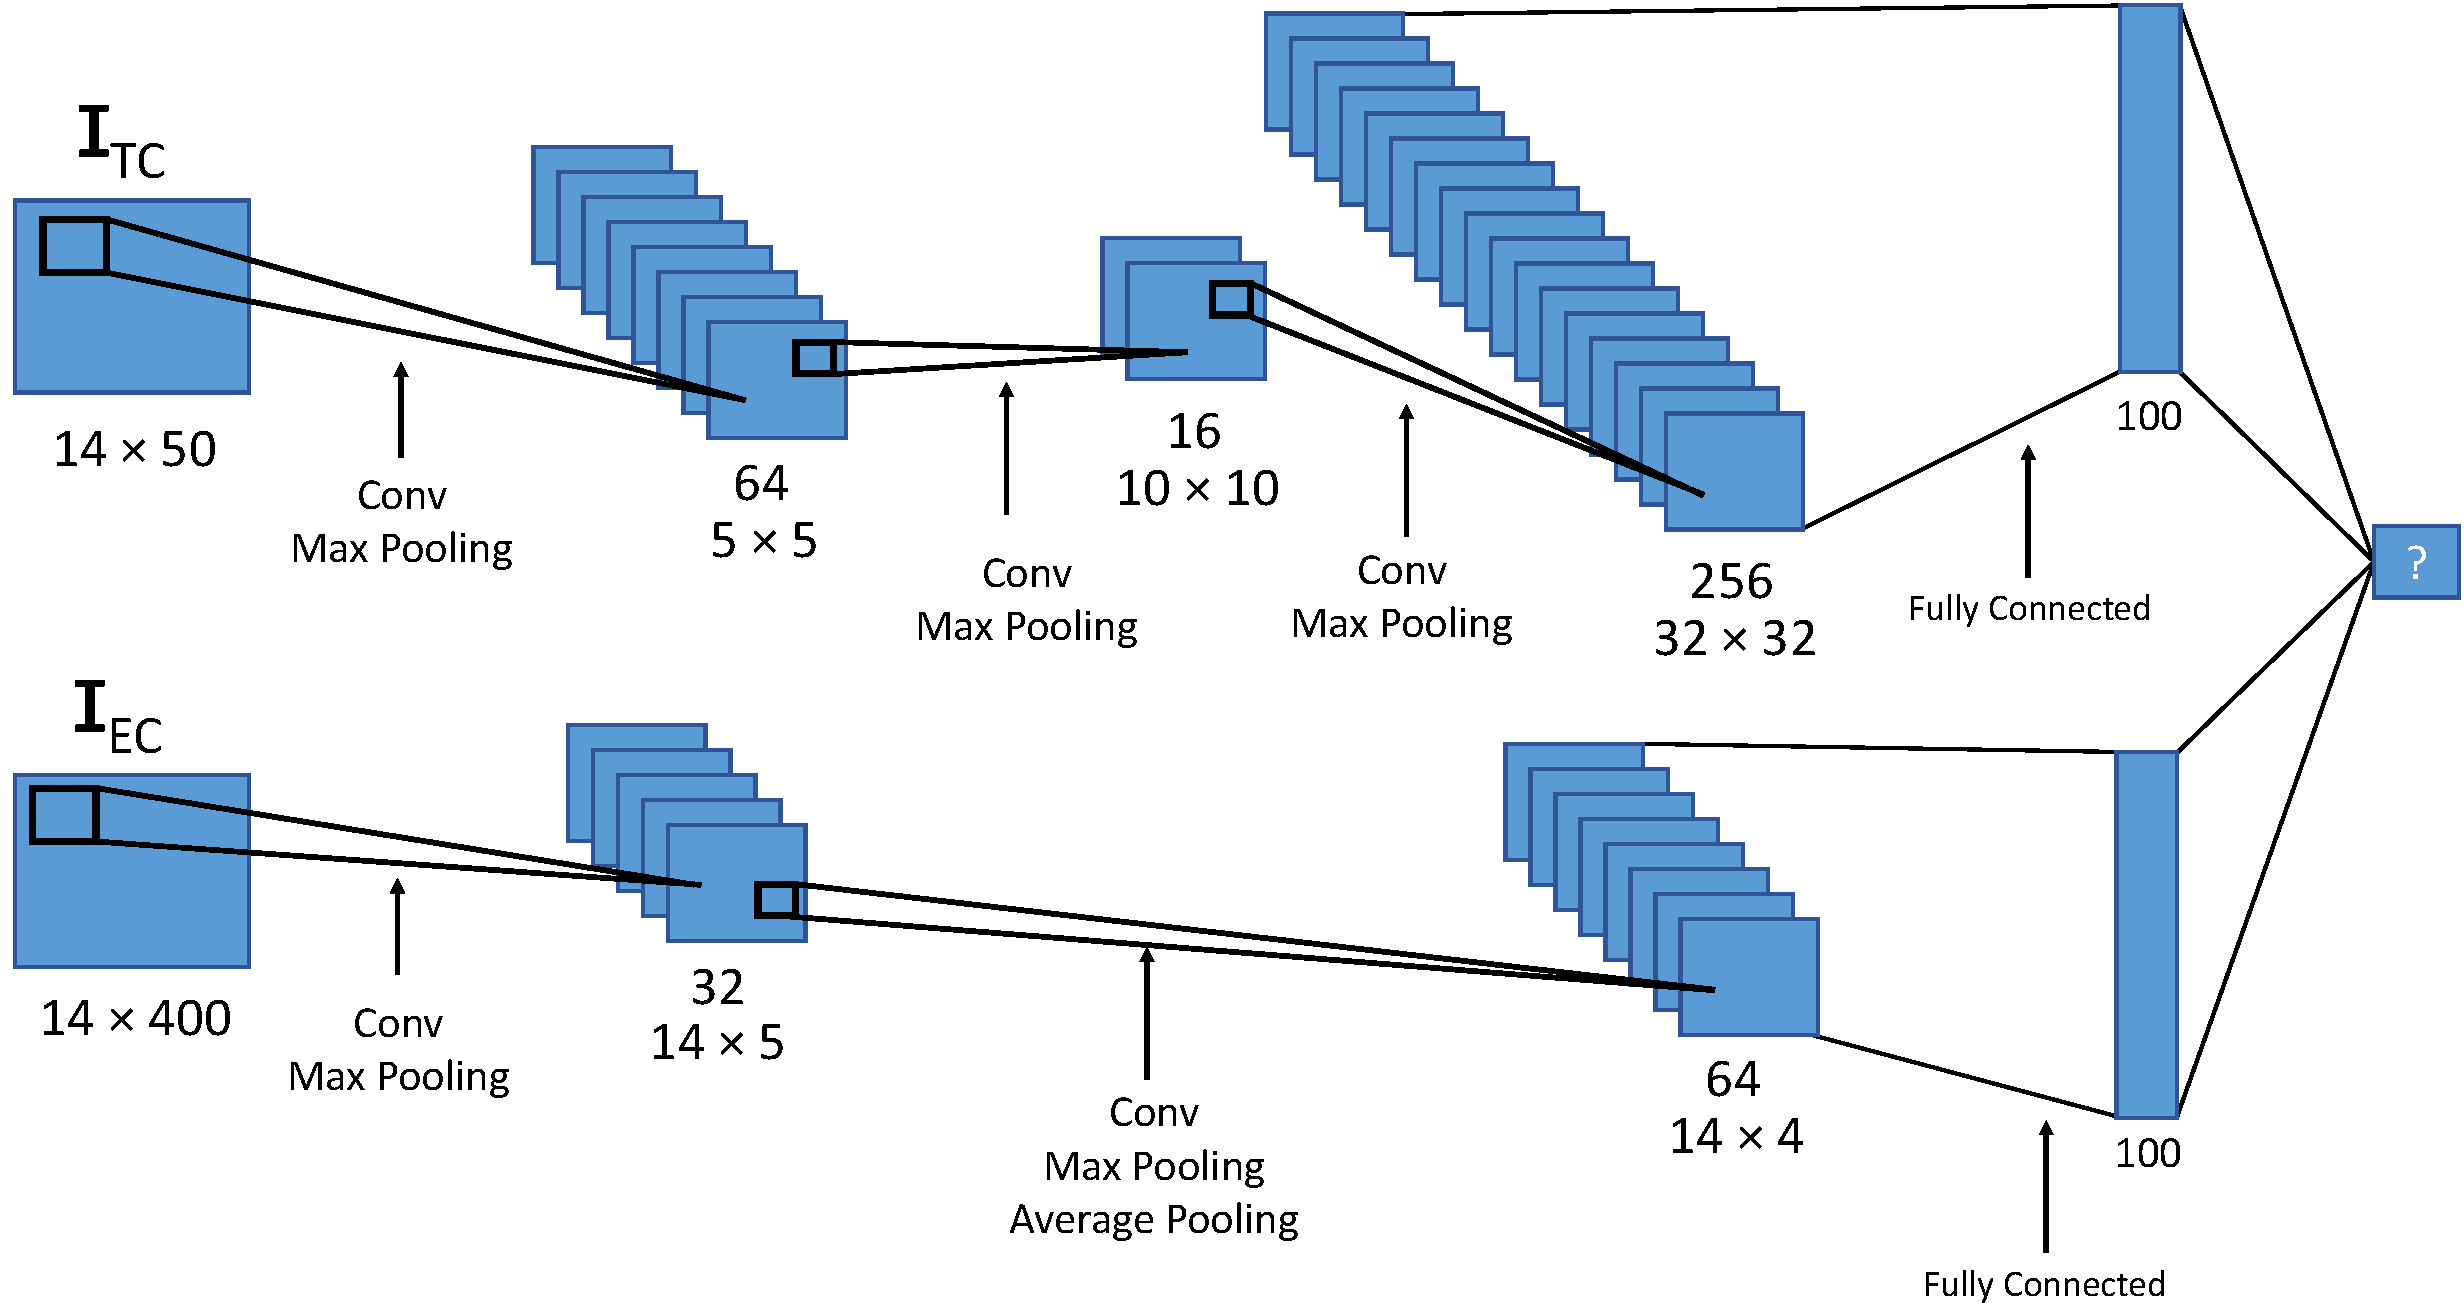
\includegraphics[width=\textwidth]{model_vis1.pdf} \caption{propose model structure}\label{proposeModel}
\end{figure*}
